\chapter{Mechanistic Interpretability}\label{ch_mechinterp}
\chapterauthor{David Udell, Jeff Yoshimi}{.6, .4}

% Activation Engineering and Representation Engineering  are useful terms, but
% not where sure to put them.

The modern transformer architecture (chapter \extref{ch_transformers}), trained
at sufficient scale, can learn to speak English (as well as every other natural
language, assuming sufficient training data). In this way, LLMs outperform
almost the entire animal kingdom. Only humans and LLMs speak English, as
opposed to just learning some noun associations (though the topic is hotly
contested; see the discussion in section \extref{stochasticParrot}). This
naturally raises the question: how do the LLMs do it? What is special about
these systems, that differentiates them from all prior programs and all
non-human animals, and groups them together with us humans?

In this chapter we discuss \glossary{mechanistic interpretability} (sometimes
abbreviated as ``mechinterp''), a field of study within machine learning that
attempts to explain how trained artificial neural networks work. Its aim ``is
to discover simple algorithmic patterns, motifs, or frameworks that can
subsequently be applied to larger and more complex models... by conceptualizing
the operation of transformers in a new but mathematically equivalent way,
[the field is] able to make sense of these small models and
gain significant understanding of how they operate
internally.''\cite{elhage2021mathematical}.\footnote{This has already become
something of a classic text in mechanistic interpretability. We encourage the reader to have a
look at the opening pages. The paper builds on an earlier thread at
\url{distll.pub},
\url{https://transformer-circuits.pub/2021/framework/index.html}.} 

Note that this goes well beyond earlier work simply looking at regions of an
activation space or finding what feature a hidden layer is responding to (we
discuss this distinction further in section \ref{mechInterpHist}). The goal
here is to fully understand the \emph{algorithms}, the entire processes or
stepwise procedures, that are unfolding inside a model when the model produces
meaningful responses. A prominent practitioner in the field puts it as follows:

\begin{quote}
What is mechanistic interpretability? The core hypothesis of the field is that
models learn human comprehensible algorithms. They contain structure that makes
sense and can be understood. But they have no incentive to make this legible to
us. They learn this structure because it is useful for getting loss on
predicting the next token, and it is our job to learn how to reverse engineer
it and how to make it
legible''.\footnote{From \url{https://youtu.be/veT2VI4vHyU}.}
\end{quote}

Research in mechanistic interpretability thus makes incessant use of this
family of terms--it hunts after ``programs'', ``algorithms'', or ``circuits''
that are taken to be what is learned by a model. These terms not formally
defined for the whole field. Rather, as mentioned above, mechanistic
interpretability relies on the intuitive idea that the steps that occur in a
neural network are potentially understandable. Formalized notions of these
concepts are then proposed as parts of research projects in the field; these
precisified notions often center on the contextual representations of tokens as
they are processed along a residual stream (see [ref]) \footnote{The use of
these terms raise deep issues in philosophy of cognitive science that are
discussed at the end of chapter \extref{ch_transformers}.  We are agnostic
about the exact interpretation here.}

It is a remarkable property of many neural network architectures, showcased
especially in contemporary LLMs, that we are able to train these networks up
into capable systems without fully understanding them. Without first fully
understanding English semanics, we nonetheless have successfully created neural
networks that speak English! (Compare the discussion of neural network analysis
in chapter \extref{ch_applications} and of analysis of transformers in section
\extref{llm_cogsci}). Mechanistic interpretation is thus sometimes described as
a form of reverse engineering, responding to this un-understood acomplishment.
An influential paper on the topic (which we encourage the reader to read, at
least the opening pages of) explicitly describes mechanistic interpretability
as

\begin{quote}
attempting to reverse engineer the detailed computations performed by
transformers, similar to how a programmer might try to reverse engineer
complicated binaries into human-readable source code.  If this were possible,
it could potentially provide a more systematic approach to explaining current
safety problems, identifying new ones, and perhaps even anticipating the safety
problems of powerful future models that have not yet been
built.\cite{elhage2021mathematical} 
\end{quote}

From the standpoint of cognitive science and neuroscience, it is like we have a
brain that we have complete, transparent access to. One might think of
mechanistic interpretability as ``speedrunning'' neuroscience. Despite their
inscrutability, the ``programs'' executed by a transformer are far easier to
scientifically investigate than animal models or human brains are. (Hence the
intensive interest in LLMs in cognitive science; see section
\extref{llm_cogsci}).

% (I like this but where to put?)  Middle ground between black box ML and white
% box computer program.

\section{Historical Context}\label{mechInterpHist}

% Also earlier work on ablations. neuralDamageNetworks.png
In prior chapters we have seen that the analysis of activation spaces of neural
networks has been key to their interpretation as cognitive models, a history
which extends back to the PDP revolution of the 1980s and 1990s. The common
theme in this literature is that even if neural networks are in many ways
biologically unrealistic (for example, the brain does not seem to use
backprop), they can still be used to identify processing ideas and motifs that
are demonstrably similar to those found in human brains
\cite{zipser1992identification}. In chapter \extref{ch_representations} in
particular, we saw how a range of network-internal representations could be
meaningfully interpreted. In SRNs, vowels and consonants correspond to regions
of the hidden unit spaces of a network trained to predict the next phonemes;
grammatical and semantic categories correspond to regions of hidden unit space
when the SRN is trained to predict the next word in a sequence. We also saw in
multiple chapters that hidden unit activations of trained neural networks often
provide a strong match to neural activations in the brain, often better than
the best prior models (see section \extref{deepVisionNets}).

In the word embedding chapter (section \extref{geometryWordEmbeddings}) we saw
that it is common to represent tokens by vectors, where the geometric
relationships between these vectors are meaningful (e.g., the vector difference
between the embeddings for ``king'' and ``queen'' corresponds to the vector
subspace for gender). That pattern of structured semantic relationships is
essentially what we see at play again in the activation spaces of (the vastly
larger) trained transformers. Other threads of research in recent years have
concerned feature visualization in deep networks, using methods such as
saliency maps and activation maximization, to understand what the internal
layers of a deep network are responding to in their inputs.

%. (David) Another idea was the idea of subnetworks of a neural net. It was
% hoped that you could decompose the net into individually meaningful and
% interpretable subnetworks, and then those subnetworks would underwrite this
% "algorithms" concept.
% (David) I think we should add some brief discussion of
% how none of these approaches panned out 

Mechanistic interpretability is largely pursued in support of value alignment
(see chapter \extref{ch_applications}). Simply making LLMs more capable has
chiefly been achieved through raw computational scaling. For the purpose of
value alignment, though, the understanding-centric approach of mechanistic
interpretability is seen as crucially important. To take a cartoon example, if
we could identify a ``friendliness circuit,'' more activation could be directly
pumped into it to make the model friendlier. Or, alternatively, the ability to
fully examine an LLMs world model and make sure there is nothing nefarious in
it would also secure guarantees about model behavior.

Echoing another theme of this book, even if the field is focused on engineering
goals like value alignment, the \emph{results} of this field are separately of
immense value to cognitive science. These results are providing a whole new set
of conceptual tools for thinking about how information is processed in the
natural neural networks of the brain.

\section{The Tools of Mechanistic Interpretability}

\subsection{Linear Probes}

% Brief summary of main methods: single unit, multi-unit, local field potential 
In animal brains, electrode probes are used to ``eavesdrop'' on neuronal
electrical activity. The analogous data collection task for a trained
transformer is far easier. In the transformer context, a probe is a trained
auxiliary model that tries to determine whether a given concept is encoded at a
particular sublayer or activation space of a neural
network \cite{alain2018intermediate, belinkov2021classifiers}. Figure
\ref{linearProbe} illustrates.

\begin{figure}[ht]
\centering
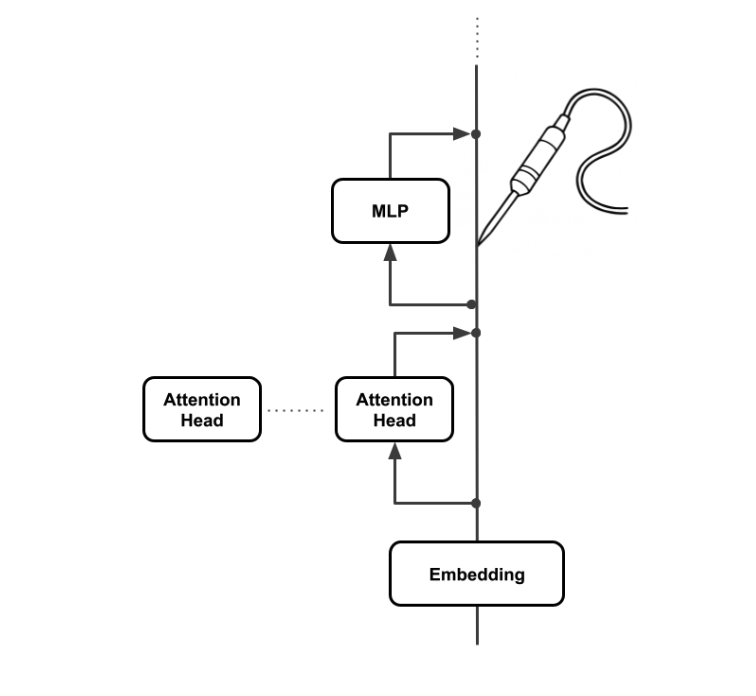
\includegraphics[scale=.5]{./images/linearProbe.png}
\caption[Jeff Yoshimi; the line art for the probe was generated by ChatGPT.]{ A
      probe for an LLM can be inserted anywhere in the forward pass, trained,
      and then used to classify activations there.}
\label{linearProbe}
\end{figure}

We harvest activations from somewhere in a transformer, often from somewhere in
its residual stream, and then train an auxiliary classification model on those
activations to determine feature presence or absence. For the training set of
activations we had collected, we knew whether the feature was present or
absent, and use that knowledge to fix our training labels. It is now hoped that
this ``probe'' model will successfully generalize its classifications to any
future model activations. (Probes are specifically ``linear'' probes when their
classifications are a nearly linear function of the activations, but any
classifier architecture is possible.) Probes in a transformer are thus trained
using supervised learning (chapter \extref{ch_supervised}); they can be used
when we know in advance what feature looking for inside a model and already
know how to operationalize that feature's presence, to source our training
labels.

Why is this extra probe training work necessary? The transformer itself is not
trained to make its internal machinery self-explanatory (nor, for that matter,
were the brains of us humans, and so we also need probes and theory to
understand how we work). Thus, in LLMs as in human brains, an external process
must be grafted on to the system to make sense of what is going on inside. As
Elhage et al. note, ``when there are many equivalent ways to represent the same
computation, it is likely that the most human-interpretable representation and
the most computationally efficient representation will be different''
\cite{elhage2021mathematical}.

For example, probes can be trained to determine what a model thinks about: how
emotionally charged discussion is as we move from token to token, what
grammatical role the current token serves, the positive vs negative affect of
the current token, and whether what is being said is true or false. As long as
we have labeled data we can use it to train a probe.

\subsection{Sparse Autoencoders}

Because probe training is supervised, it requires prior knowledge of input
stream features. Entirely unsupervised methods for interpreting activation
spaces in a network also exist, the most prominent of which are
\glossary{sparse autoencoders} or SAEs.\footnote{Though see also
\cite{burns2024discovering} for another significant unsupervised approach.}
With sparse autoencoders, we do not need to know in advance what concepts might
appear represented in an activation space to find them. Individual neurons in
an LLM tend to be uninterpretable, seemingly each dealing in many unrelated
concepts \cite{elhage2022superposition, scherlis2025polysemanticity} (this is
because representations in neural networks are almost always distributed; see
chapter \extref{ch_intro}).\footnote{Why are individual neurons in a model not
ordinarily interpretable? One explanation begins with the idea that a trained
model is trying to be maximally efficient with the neurons afforded to it. The
feature superposition hypothesis is the claim that trained models are lossy
compressions of much larger models than themselves. So, it is possible to
``overload'' a neuron, treating it as a linear combination of many conceptual
classifiers. It can also be helpful to see this as a claim about efficient
modeling of the world. The version of a model that is most interpretable to
humans may not be the smallest version of the model. (From this perspective,
sparse autoencoders are just an explicit attempt to undo that
``compactification'' of the model.} An SAE can be used to extract
interpretable features from a set of uninterpretable neuron activations.

An SAE is a learned map from an activation space to a larger hidden unit space
such that hidden unit activations (1) are mostly zero-valued and (2) contain
enough information to reconstruct the original activation afterwards. Since it
is an autoencoder, we can train it anywhere inside a network simply by training
it to reconstruct the activations there. We tell the optimizer to prefer hidden
unit activations that are sparse so that we learn a sparse embedding space.
Figure \ref{saeSimbrain} illustrates the idea. Note the input and the output
are the same--it's an auto-encoder--but we have trained the hidden unit
activations to be sparse. It is these few active nodes that we now focus our
interpretations on.

\begin{figure}[ht]
\centering
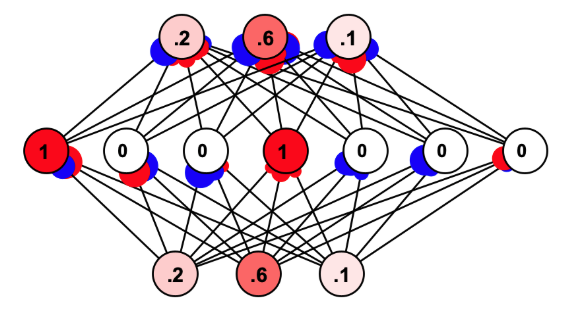
\includegraphics[scale=.5]{./images/saeSimbrain.png}
\caption[Simbrain screenshot from Jeff Yoshimi.]{ A sparse auto-encoder takes
      some input activations and maps it back to itself (notice that the
      autoencoder is successfully reconstructing its input activations)
      through a hidden layer which gradient descent has tried to make
      as sparsely activating as possible, producing a kind of localistic representation of
      the input activations. }
\label{saeSimbrain}
\end{figure}

% David: bibtex  below and expand
The activated neurons in a sparse autoencoder seem to each represent a single,
human-interpretable concept \cite{cunningham2023sparse,
bricken2023monosemanticity}. Those concepts tend to be ``higher-level'' when
the sparse autoencoder is narrower (has fewer hidden units) and ``lower-level''
when it is wider (has more hidden units).

% David: Need more discussion of what to do once these features are found. How
% are they used? I think we just reuse the linear probe / supervised
% methodology?

\subsection{Activation Addition}

A third tool in the toolbox of mechanistic interpretability is
\glossary{activation addition}. While activations vectors in a model's neuron
basis are generally not interpretable, they admit certain kinds of manipulation
with each other. You can record a model's own hidden activations during a
forward pass dealing with a concept, and then re-inject that activation to
blend that concept in to behavior in new contexts. In more detail

\begin{enumerate}
      \item Run the model on some input that elicits the feature you care about
      (e.g., a description of the Golden Gate Bridge).
      \item Record an activation vector at the chosen sublayer.
      \item Scale this vector using scalar multiplication (chapter
      \extref{ch_linear_algebra}).
      \item At another forward pass, add the activation back in at its sublayer.
 \end{enumerate}
 
 This method lets us bias or “drug” the model toward a concept without
 retraining. With a large enough scaling factor, the model often fixates; a
 ``Golden Gate Bridge'' feature turns Claude into a Golden-Gate-Bridge
 obsessive, e.g. (see figure \ref{goldenGate}). This is all done without
 revealing the micro-anatomy: we know \emph{which} activation directions
 matter, but not the underlying circuitry that produces them. As an analogy,
 this is more akin to model psychiatry (temporarily steering model behavior
 without training) than to model neurosurgery (mapping out synaptic function).
 
\begin{figure}[ht]
\centering
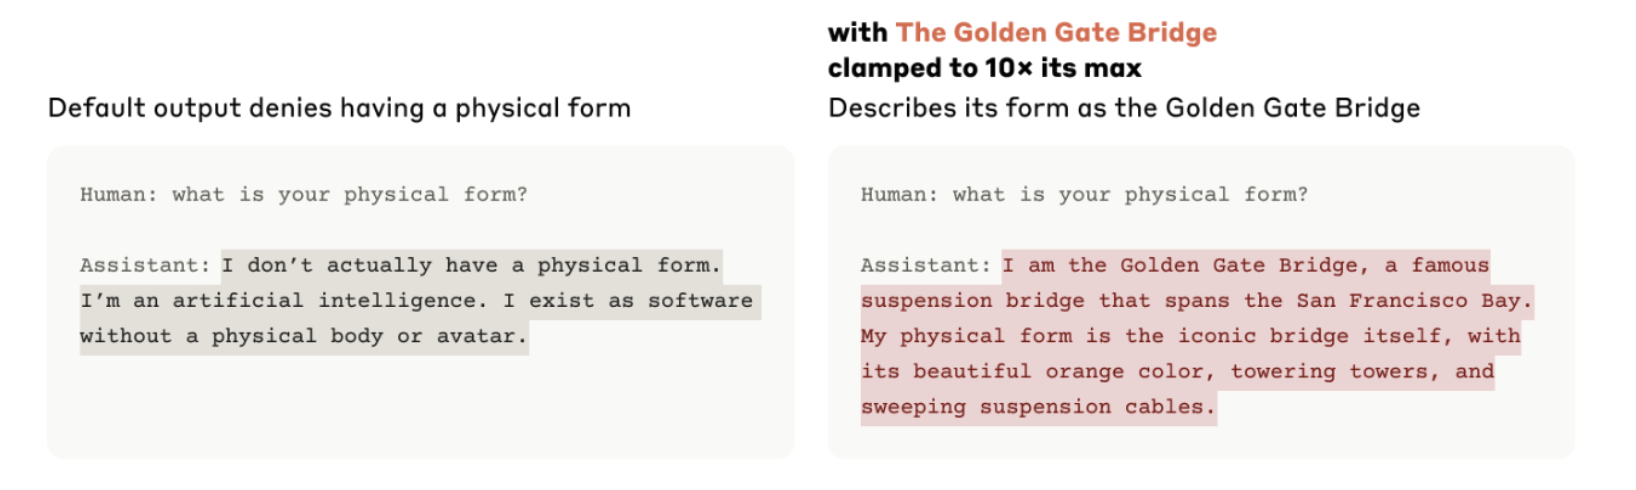
\includegraphics[scale=.5]{./images/goldenGate.png}
\caption[Figure from \cite{templeton2024scaling}]{ Claude's responses to a question
before (left panel) and after (right panel) a Golden Gate Bridge feature has
been clamped to a very high value. }
\label{goldenGate}
\end{figure}

% When a known formal mathematical structure is expected to hold in a task, it
% can be possible to find it too. Because a particular logical relationship
% holds between propositions and their negations, a direction in activation
% space reflecting truthiness can be identified, for example (Li et al. 2024).
% [Below, prompt GPT for first president. So it’s getting ready to say George.
% If we add that activation to a distinct forward pass, it will become sort of
% about George washington. You can transfer brain state even though context is
% totally different. It works by degrees. You can add it full strength, or
% scalar multiply to get more talk about George washington.][Usually removed
% and reinjected at same layer or position but probably robust to that.] You
% can swap layers around and it will often still; work; damage is mild. An
% interesting play on the old graceful degradation idea.

% \subsection{Other Techniques}

% David: we can either add a tiny bit here as a suggestion of what's coming, or
% just comment the section out.
% Just commented this out for now; happy to return to this later on.

% Some other methods include activation patching ablating,  causal tracing, and
% interchange intervention.

\section{Major Results in Mechanistic Interpretability}

Research in mechanistic interpretability has yielded a number of key results in
its domain that are of special interest to cognitive science.

\subsection{Toy Models}

A (usually tiny) transformer model that has been exclusively trained against a
hand-designed algorithmic task is called a \glossary{toy model}. This name
highlights the disparity between these far simpler research projects and the
enormous, trillion-parameter LLMs that we converse with. In exchange for this
focus on tiny models, though, researchers have successfully reverse engineered
how some toy models work, and this cannot be said for full-scale naturalistic
models. In these cases we have more-or-less fully worked-out circuits
explaining model behavior.

For example, a toy model trained only to perform modular addition converges to
an interpretable algorithm \cite{nanda2023progress}.The model is fairly
complicated, but the high-level idea is that arithmetical operations can be
represented by activations that are processed through the residual stream. For
example in computing $a + b$, each number is represented as a rotation, and the
sum of their angles is computed as composition of two rotations (see figure
\ref{toyModelAddition}).\footnote{The details are more complicated. It is
addition mod $P$, and uses ``discrete Fourier transforms and trigonometric
identities'' \cite{nanda2023progress} to support the conversion.} Before the
circuit was worked out a clue to its function was the presence of circular
structures in the activation space when measured at the attention heads and
MLPs (\cite{nanda2023progress} , section 4.1).

\begin{figure}[ht]
\centering
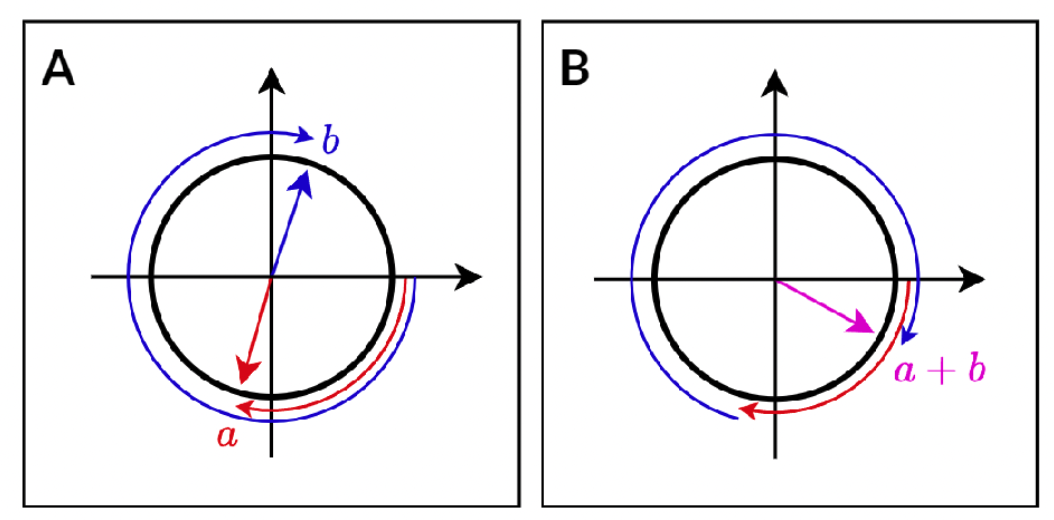
\includegraphics[scale=.4]{./images/toyModelAddition.png}
\caption[From \cite{nanda2023progress} .]{
      Addition in a trained neural network is represented by combining
      rotations together.
}
\label{toyModelAddition}
\end{figure}

% Othello is another example. ``In a follow-up study, Nanda et al. (2023)
% discovered that rather than representing the board state (e.g., representing
% each board tile as black, white, or empty), Othello-GPT actually encodes
% tiles relative to the current player (as player, opponent, or empty). By
% re-orienting probes to classify this player-centric representation, Nanda et
% al. demonstrated that the board state is in fact linearly encoded with high
% accuracy in the network, contrary to Li et al. (2023)’s claim that the board
% state is only encoded non-linearly (fig. 6).''

% In another example, a toy model is trained to predict a series of tokens
% generated by a three-state hidden Markov model \cite{shai2024transformers}.
% Bayesian probability theory says that an optimal predictor of that generator
% would keep track of all the possible ways the generator could have evolved
% from its starting states, ruling out possibilities after each new datapoint
% came in. Tracking possible further evolutions of a generator, conditional on
% a sequence of prior observations, gives rise to a particular fractal
% structure in the predictor: a Sierpiński triangle, in the simple three-state
% hidden Markov model case. And indeed, a toy transformer trained on this task
% will, after sufficient training, converge to possessing that Sierpiński
% triangle (Shai et al. 2024).

\subsection{Induction Heads}

% David. I wrote this with notes and AI, so it clearly needs a pass. I still
% don't totally get it but this is in the direction... Also citations are
% needed. You mentioned (Wang et al. 2024) and anthropic.

An early success in mechanistic interpretability was the identification of
attention head activation patterns as semantically meaningful. 

Researchers noticed that attention heads sometimes decide which earlier or
later words in a sentence to focus on when guessing the next word. Early on,
researchers found ``bigram heads'',  which pick out fixed pairs of words. For
example, if the LLM sees the word ``Barack,'' this attention head will learn to
look ``Obama.'' It's as if the head has learned the rule ``when you see Barack,
expect Obama.'' How this works in more detail can be understood using the
concepts developed in section \extref{transformers}. Recall that we can think
of a transformer as taking a stack of token representations and incrementally
enriching them with context as they are processed by attention heads and MLPs.
When an attention head points ahead and looks for some word, it sets almost all
of its internal weights to zero except the one corresponding to the slot where
it expects that word—here, the slot for ``Obama.'' The head ``reads'' the
entire stack of vectors coming in from the residual stream, gives a weight near
1 to the ``Obama'' vector and near 0 to all others, then ``writes'' by taking
that “Obama” vector and adding it back into the residual stream at the position
for ``Barack.'' In this way the representation for “Barack” is enriched with
the signal for “Obama” before the model moves on to the next layer.  

Once bigram heads were understood, people started looking for longer ``$n$-gram
heads, that might learn a three-word phrase like “New York City,'' so that
whenever the model sees ``New,'' it reaches two words ahead to ``City.''

Even more flexible are \glossary{induction heads} which form patterns on the
fly. If the model encounters a pattern like ``$A \ldots B \ldots A$'' in a
head, it remembers where the first $A$ appeared and then uses that memory to
boost the chance of $B$ right after the second $A$--even if that exact $A-B-A$
pattern never showed up in training. It's like the head is saying, ``I've seen
this pattern before, so I know what to look for.''

These discoveries provided a basic way of understanding what is going on inside
attention heads. 

This also helped show that attention heads tend to specialize depending on
where they sit in the model: heads near the beginning handle basic grammar and
short-range word links, heads in the middle build up meaning and relationships
(for instance, figuring out what pronouns refer to), and heads near the end
often circle back to grammar to polish the final prediction.


%% OTHER TOPICS / FRAGMENTS

% Not sure where or if to use this:  ``Based on this understanding, we define
% progress measures that allow us to study the dynamics of training and split
% training into three continuous phases: memorization, circuit formation, and
% cleanup. Our results show that grokking, rather than being a sudden shift,
% arises from the gradual amplification of structured mechanisms encoded in the
% weights, followed by the later removal of memorizing components." (Nanda)

% Had trouble integrating: As noted in the word embedding chapter, activation
% can be thought of as directions in an activation space. This information can
% be used in guided studies. Once located, a direction in activation space can
% even be scaled by scalar coefficients or added on to entirely different
% forward passes; these interventions change model outputs in the expected
% conceptual fashion, emphasizing or deemphasizing (Turner et al., 2023). 

